\begin{figure}[H]
\centering
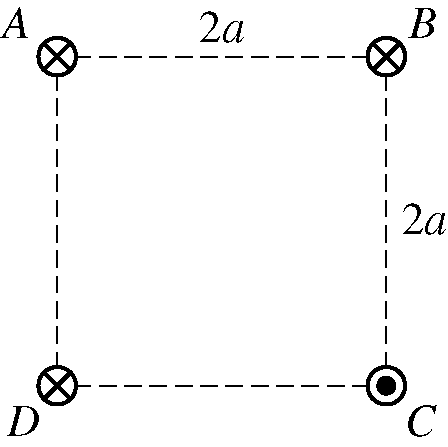
\includegraphics[scale=0.3]{images/img-012-038.png}
\end{figure}

% Multiple Choice Question 29
\begin{questions}\setcounter{question}{28}\question
Four long, straight wires are arranged at the vertices of a square with sides of length $2 a$, as shown in the figure above. Each wire carries a current $I$. The currents of three of the wires are directed into the page, while the current at point $C$ is directed out of the page. What is the magnetic field at the center of the square?

\begin{choices}
\choice $\dfrac{\mu_{0} I}{\sqrt{2} \pi a}$ toward wire $D$
\choice $\dfrac{\mu_{0} I}{\sqrt{2} \pi a}$ toward wire $B$
\choice $\dfrac{\mu_{0} I}{\sqrt{2} \pi a}$ toward the bottom of the page
\choice $\dfrac{\mu_{0} I}{2 \pi a}$ toward wire $D$
\choice $\dfrac{\mu_{0} I}{2 \pi a}$ toward wire $B$
\end{choices}\end{questions}

